% !TeX document-id = {1ab4115c-5a48-37e6-26a7-eb5f8e718844}
% !TeX TXS-program:compile = pdflatex -synctex=1 -interaction=nonstopmode -output-directory=build -jobname=p5_aionfpga_report_canzani_mueller report.tex
% !TeX TXS-program:bibliography = biber --output-directory build p5_aionfpga_report_canzani_mueller
% !TeX TXS-program:glossary = makeglossaries -d build p5_aionfpga_report_canzani_mueller
% !TeX TXS-program:view = txs:///view-pdf ./build/p5_aionfpga_report_canzani_mueller.pdf

\documentclass[final]{fhnwreport}

%% Packages
% Main packages
\usepackage[english]{babel}
\usepackage[T1]{fontenc}
\usepackage[utf8]{inputenc}
\usepackage{lmodern}
\usepackage{textcomp}
\usepackage{graphicx}
\usepackage{float}

% Useful packages
\usepackage[pdftex,dvipsnames,table,tables]{xcolor}
\usepackage{csquotes}
\usepackage{siunitx}
\usepackage{xfrac}
\usepackage{listings}
\usepackage{lstautogobble}
\usepackage[bottom]{footmisc}
\usepackage{footnote}
\usepackage{verbatim}
\usepackage[textsize=footnotesize]{todonotes}
%\usepackage{xurl}
%\usepackage{url}
%\usepackage{soul}

% TikZ packages
%\usepackage{standalone}
%\usepackage{tikz}
%\usepackage{circuitikz}
%\usetikzlibrary{arrows}
%\usetikzlibrary{calc}
%\usetikzlibrary{intersections}

% Math packages
\usepackage{amsmath}
%\usepackage{amssymb}
\usepackage{array}
%\usepackage{amsthm}

% Table packages
\usepackage{tabularx}
%\usepackage{longtable}
\usepackage{multirow}
\usepackage{multicol}
\usepackage{booktabs}

% Figure packages
%\usepackage{subfig}
\usepackage{caption}
\usepackage{subcaption}

% PDF packages
\usepackage{pdfpages}
\usepackage{pdflscape}

% Other packages
%\usepackage{xargs}

%% Settings
% Bibliography
\usepackage[style=ieee,dashed=false,urldate=comp,backend=biber]{biblatex}
\addbibresource{literature/bibliography.bib}

% Glossary
\usepackage[toc]{glossaries}
\makeglossaries
\input{header/glossary}

% Graphics
\graphicspath{{./graphics/}}

% Listings
% purple {0.776,0.584,0.776} / yellow {0.976,0.682,0.341} / orange {0.976,0.482,0.341}
\definecolor{keywordcolor}{rgb}{0.925,0.376,0.4} % red
\definecolor{commentcolor}{rgb}{0.651,0.675,0.725} % gray
\definecolor{stringcolor}{rgb}{0.6,0.78,0.58} % green
\definecolor{backgroundcolor}{rgb}{0.976, 0.98, 0.98} % light gray

\lstdefinestyle{C++}{
    autogobble,
    backgroundcolor=\color{backgroundcolor},
    commentstyle=\color{commentcolor},
    keywordstyle=\color{keywordcolor},
    numberstyle=\tiny\color{commentcolor},
    stringstyle=\color{stringcolor},
    basicstyle=\ttfamily\footnotesize,
    breakatwhitespace=false,
    breaklines=true,
    breakautoindent=true,
    breakindent=50pt,
    escapeinside={(*}{*)},
    captionpos=b,
    keepspaces=true,
    numbers=left,
    numbersep=5pt,
    showtabs=false,
    showspaces=false,
    showstringspaces=false,
    tabsize=2,
    language=C++
}


% Other
%\geometry{twoside=false}
\setlength{\marginparwidth}{2cm}
\overfullrule=5em

%% Custom definitions
% Table definitions
\newcolumntype{L}[1]{>{\raggedright\arraybackslash}p{#1}}
\newcolumntype{C}[1]{>{\centering\arraybackslash}p{#1}}
\newcolumntype{R}[1]{>{\raggedleft\arraybackslash}p{#1}}
\newcolumntype{M}[1]{>{\centering\arraybackslash}m{#1}}
\newcolumntype{N}{@{}m{0pt}@{}}

% Month
\newcommand{\MONTH}{
	\ifcase\the\month
	\or January
	\or February
	\or March
	\or April
	\or May
	\or June
	\or July
	\or August
	\or September
	\or October
	\or November
	\or December
	\fi}

% URL
\urlstyle{same}

% siunitx
\sisetup{per=fraction}



\title{\textbf{{\Huge AI High-Performance Solution \\[2mm] on FPGA}}}
\author{\textit{{\LARGE Report}}}
\date{}

\begin{document}

% Title page
\selectlanguage{english}
\pagenumbering{gobble}
\maketitle
\vfill
\begin{center}
	\begin{tabular}{>{\bfseries\large}rl}
		Degree Program	& Electrical Engineering and Information Technology \\[2mm]
		Customer		& Institute for Sensors and Electronics \\[2mm]
		Coaches			& Prof. Michael Pichler, Prof. Dr. Hanspeter Schmid \\[2mm]
		Team			& Nico Canzani, Dominik M\"uller \\[2mm]
		Date			& \the\day.\MONTH \the\year
	\end{tabular}
\end{center}
\clearpage

% Contents
\pagenumbering{roman}
\tableofcontents
\clearpage

% Sections
\pagenumbering{arabic}
\section{Section}
\label{sec:section}


% Bibliography
%\printbibliography[heading=bibintoc]
%\label{sec:literature}
%\clearpage

% Glossary
%\printglossaries
%\clearpage

% Appendix
%\begin{appendix} \todo{Drawings noch korrekt einfügen, sind nur mal drinn, um verweisen zu können.}
  \section{Problem Statement}
  \label{app:problem_statement}
  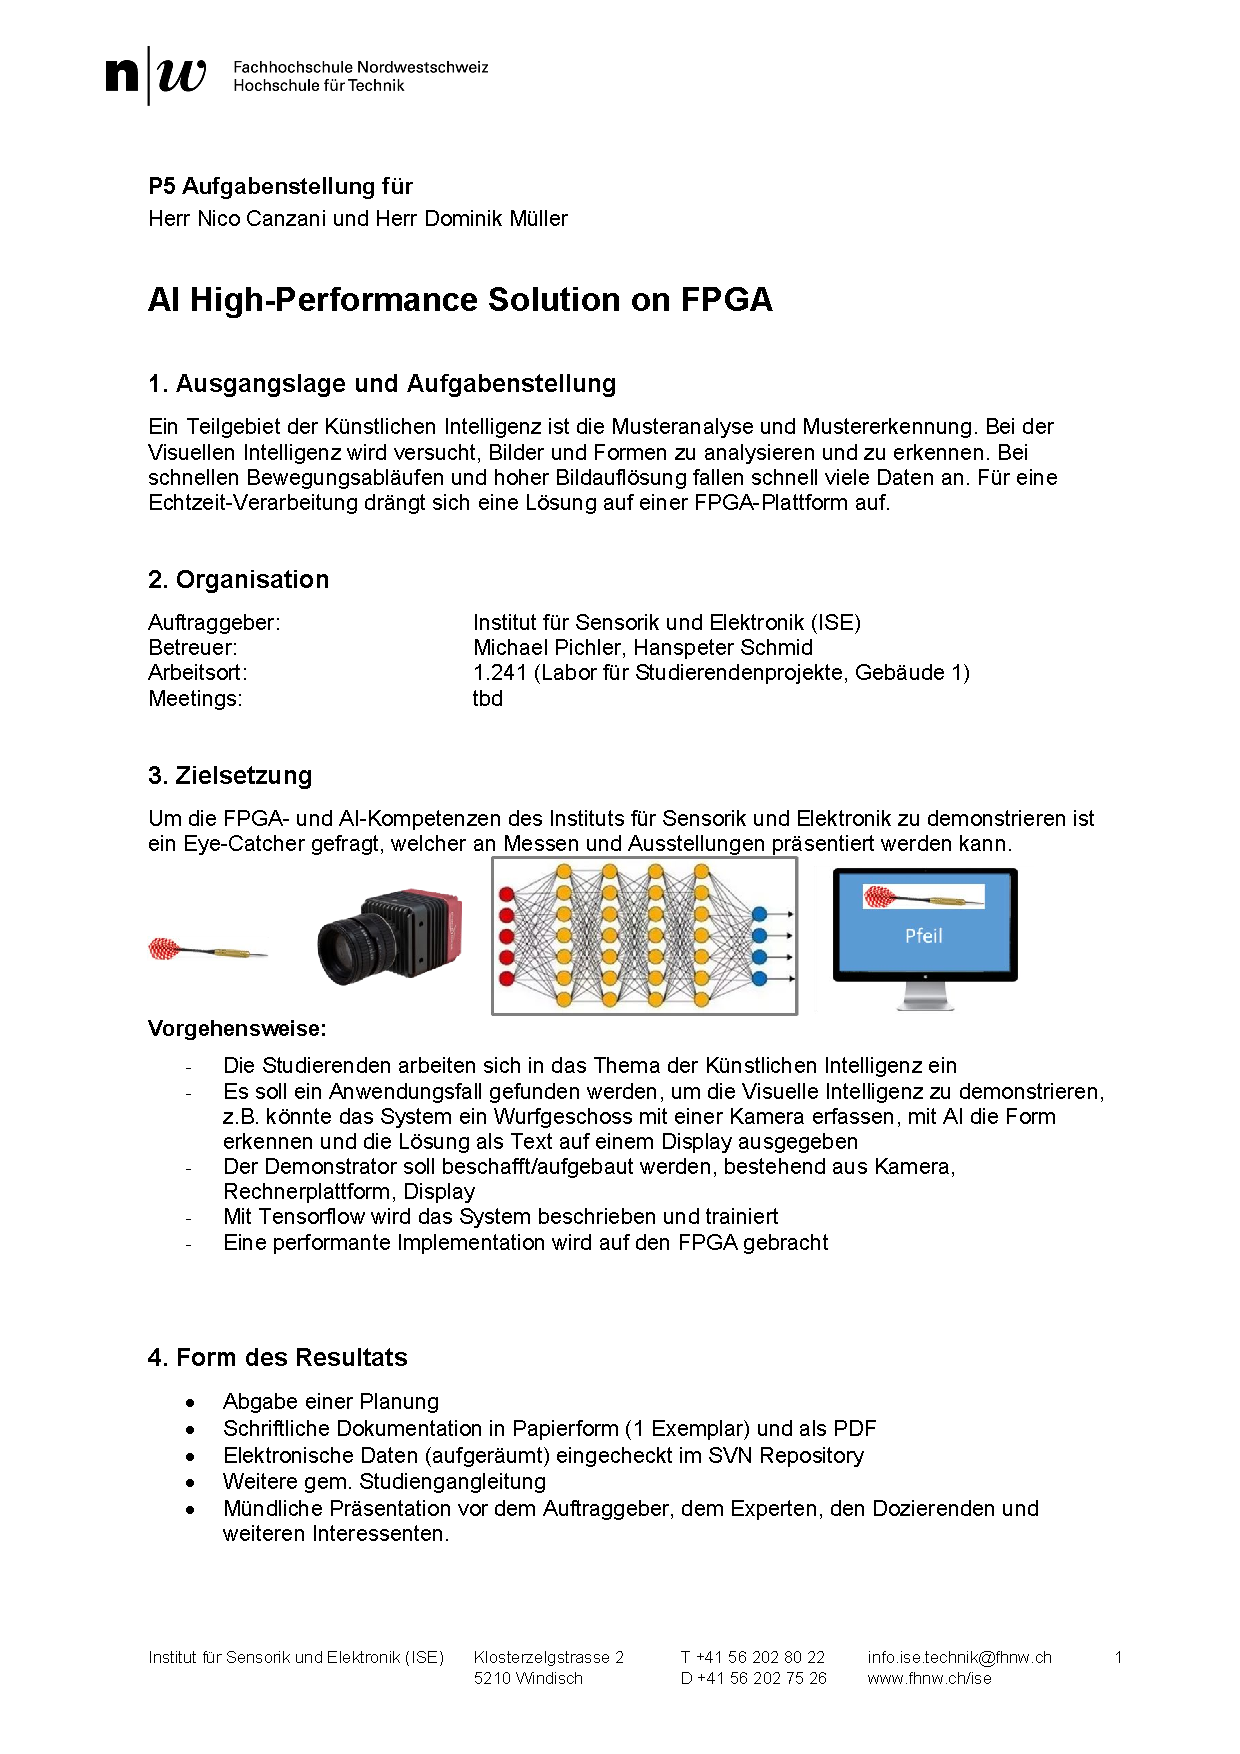
\includepdf[pages=-]{appendix/problem_statement.pdf}
  % 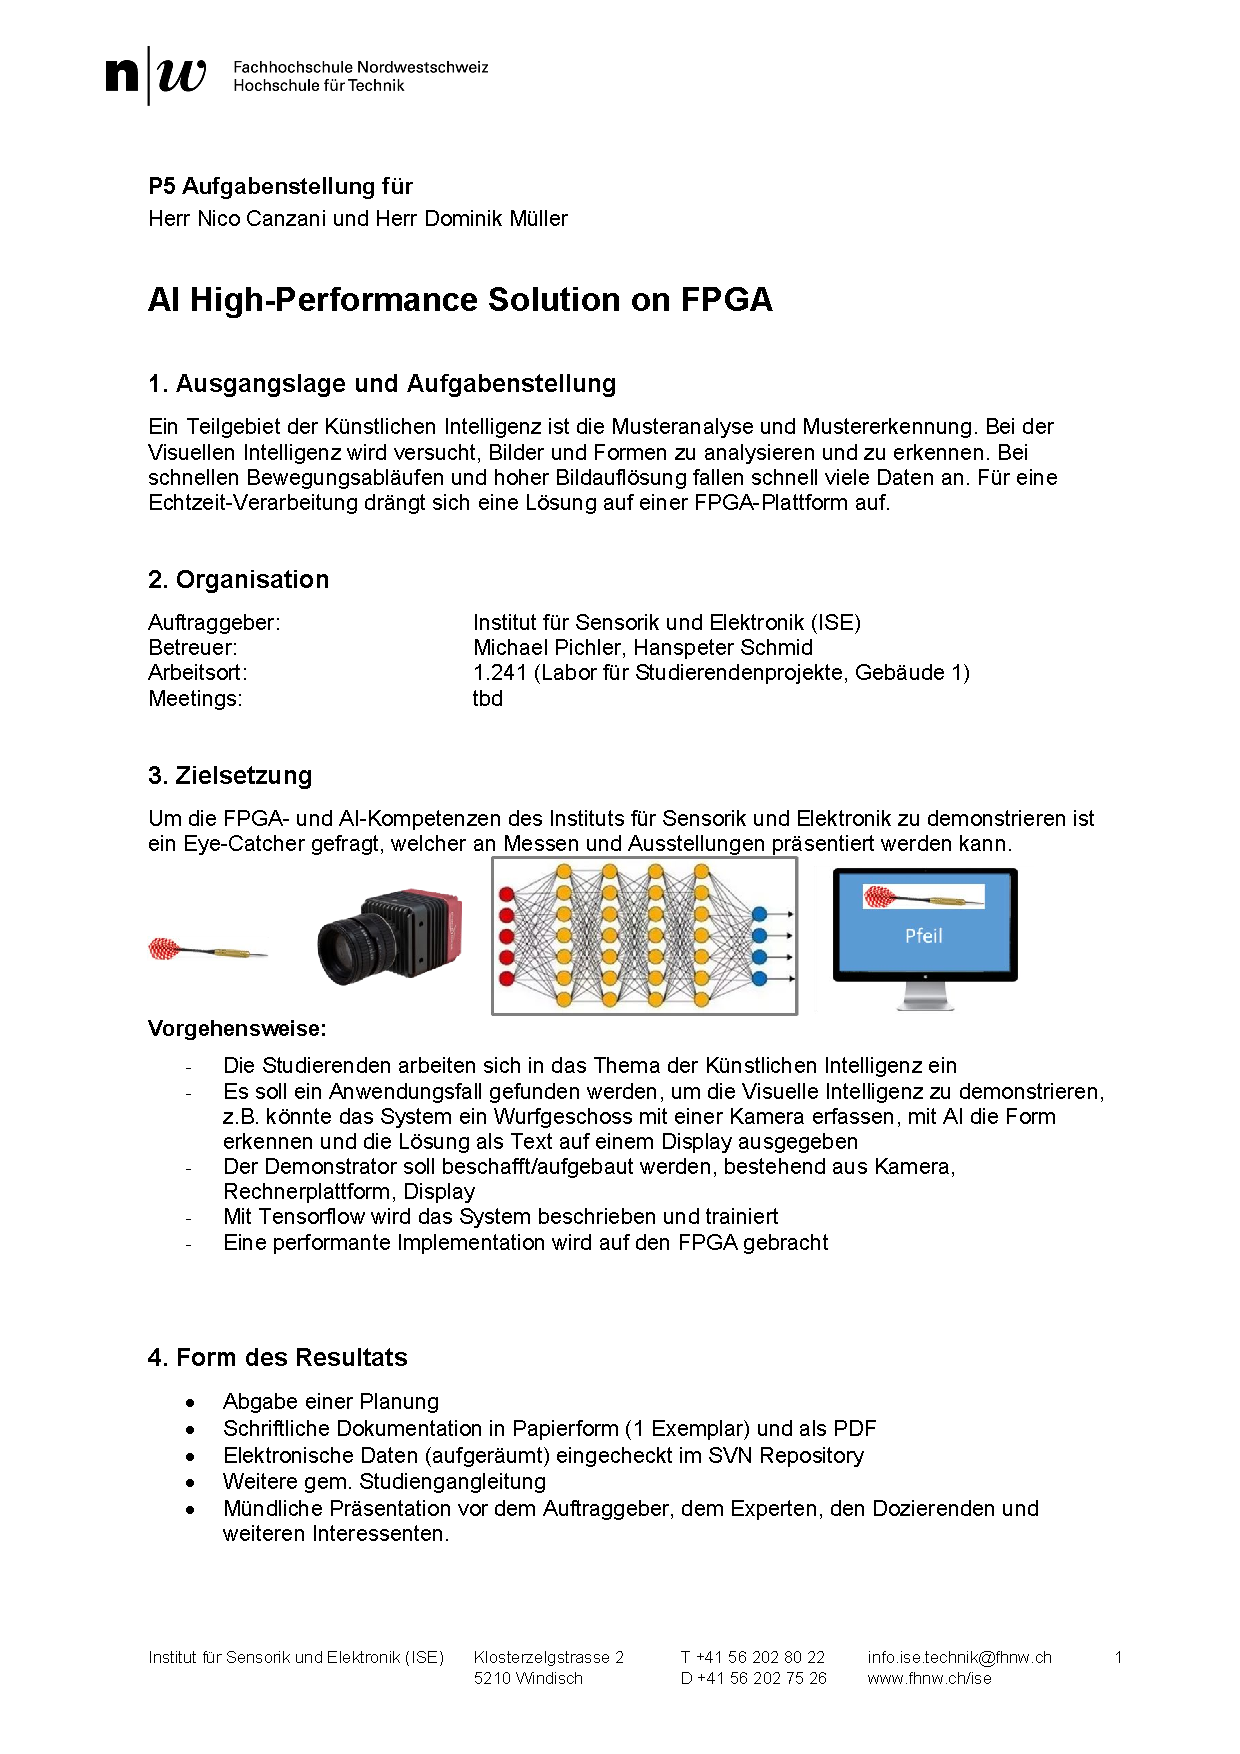
\includepdf[pages=-,nup=1x2,landscape=true]{appendix/problem_statement.pdf}

  \section{Drawing Camera Protection}
  \label{app:drawings_camera_protection}
  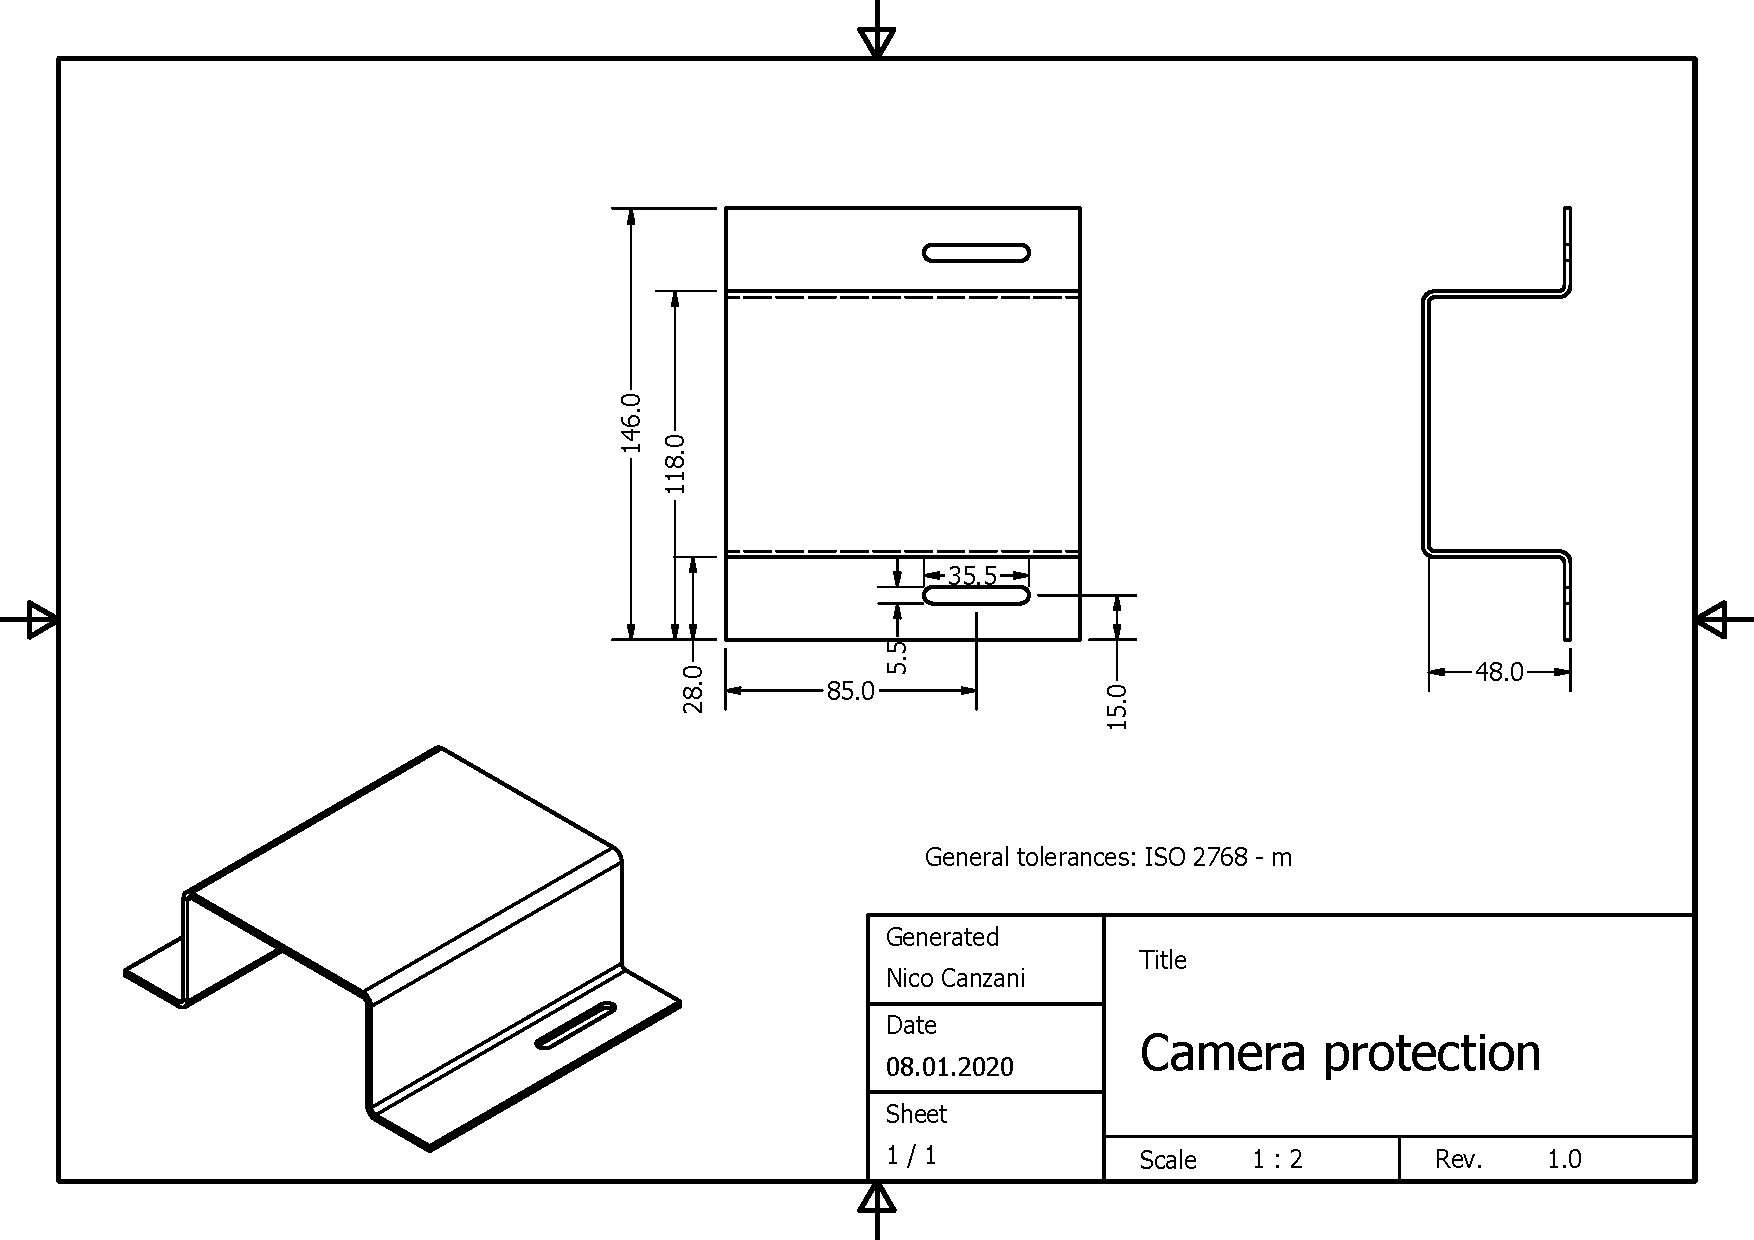
\includepdf[pages=-,landscape=true]{appendix/drawings_camera_protection.pdf}

  \section{Drawing Fibox}
  \label{app:drawings_fibox_bottom}
  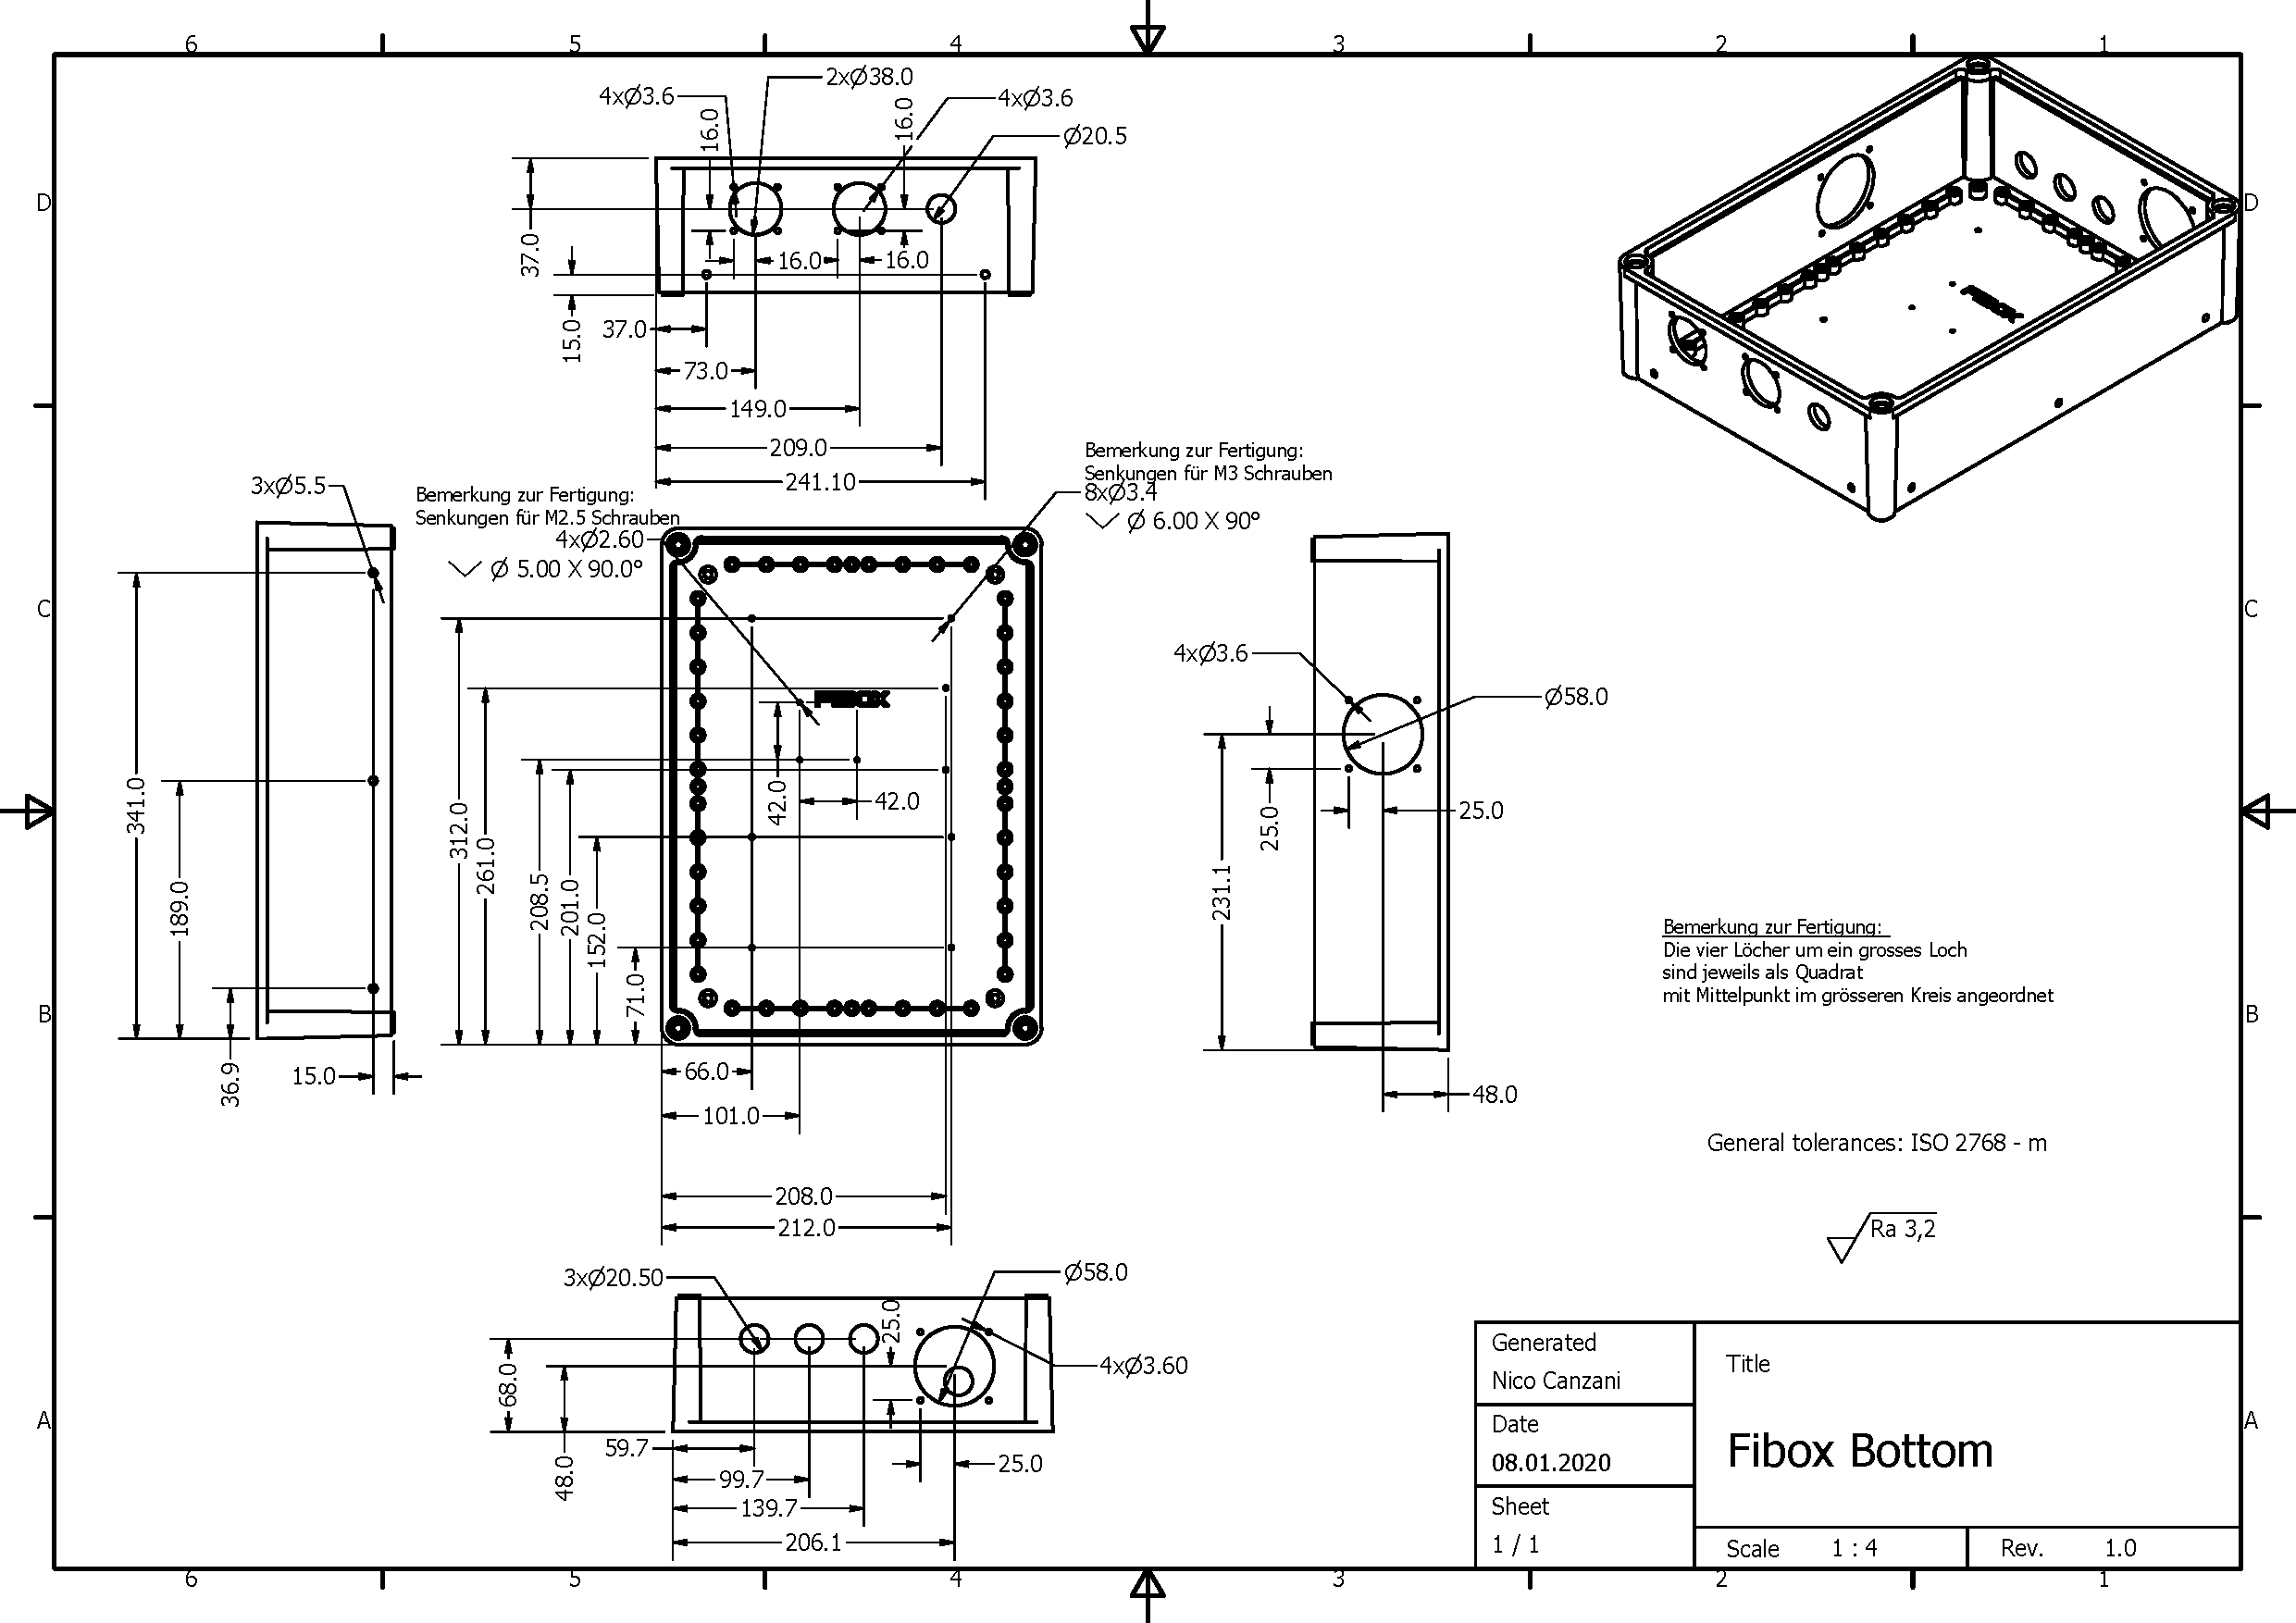
\includepdf[pages=-,landscape=true]{appendix/drawings_fibox_bottom.pdf}

  \section{Drawing Mounting Adapter}
  \label{app:drawings_mounting_adapter}
  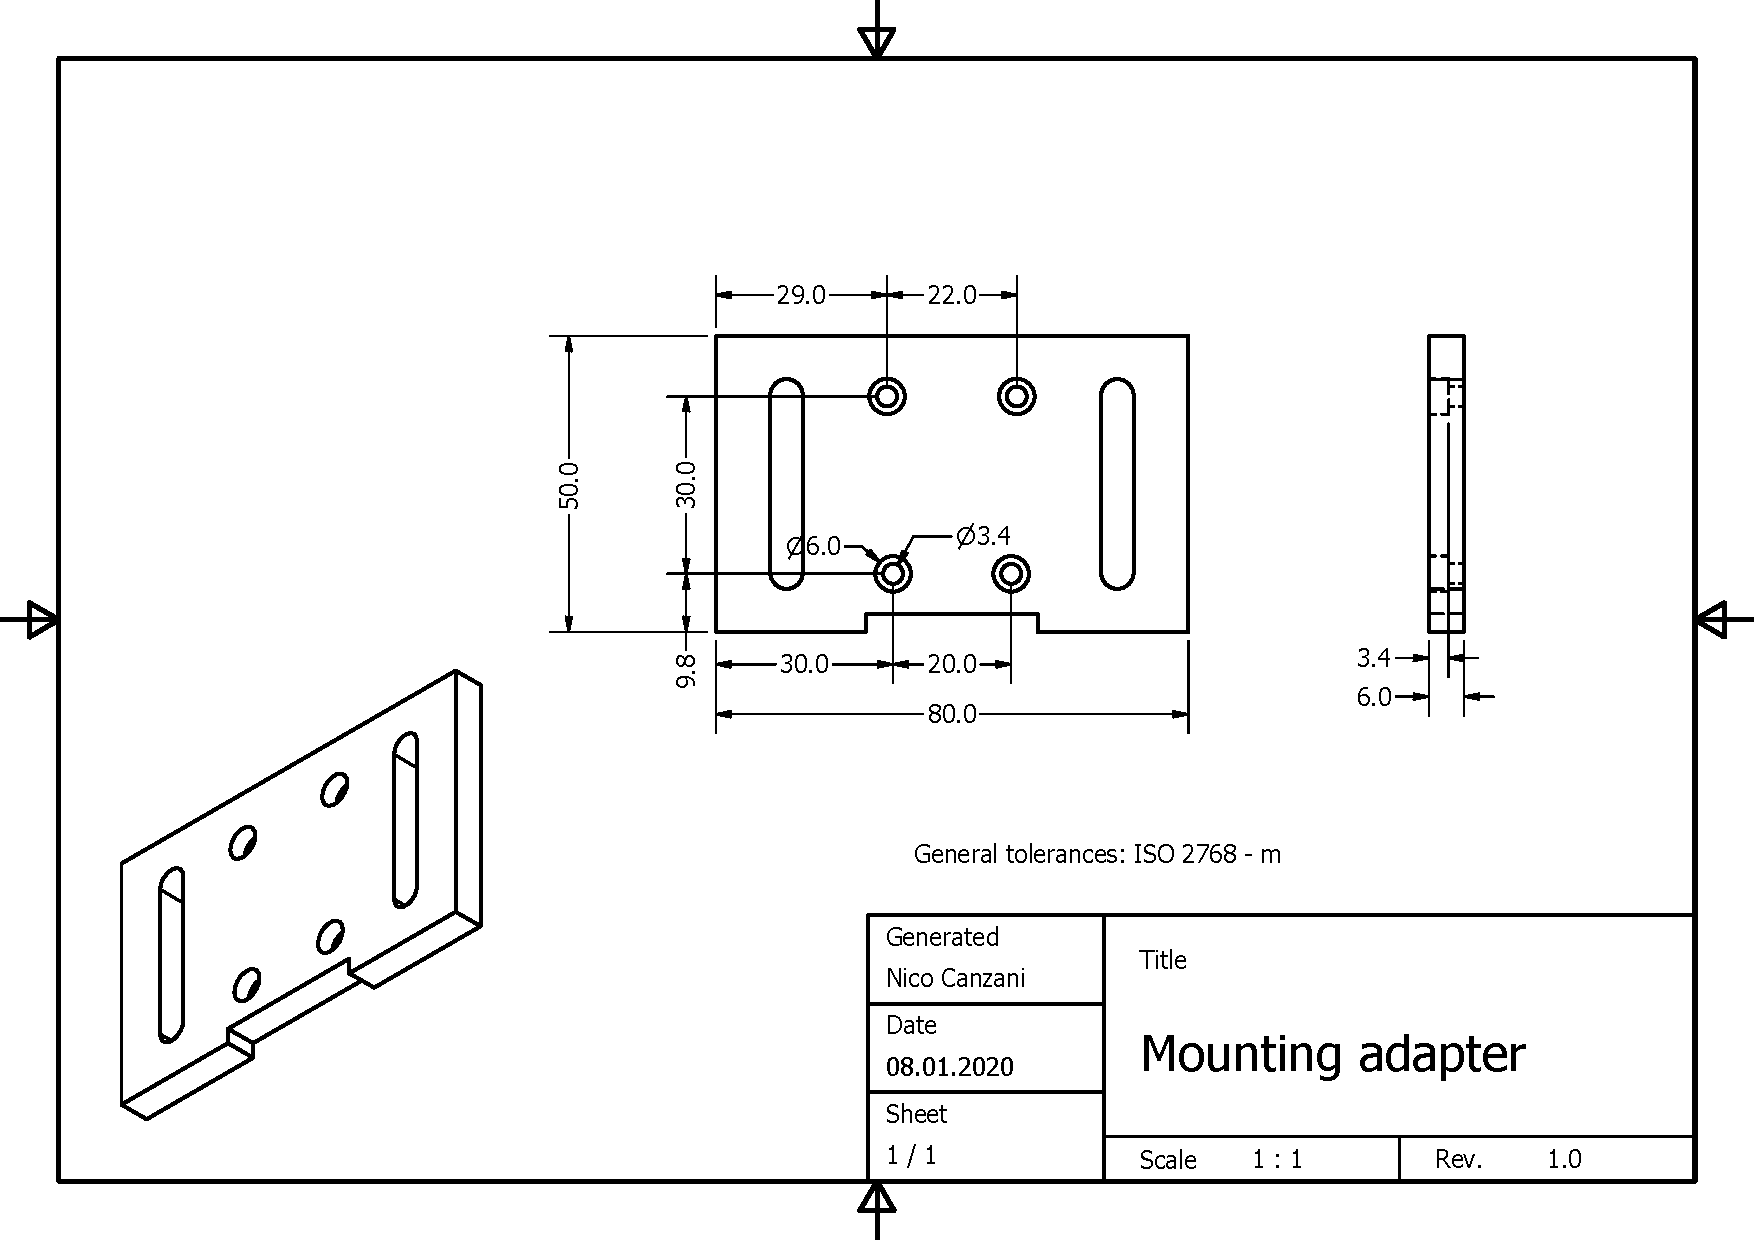
\includepdf[pages=-,landscape=true]{appendix/drawings_mounting_adapter.pdf}

  \section{Drawing Rear Panel}
  \label{app:drawings_rear_panel}
  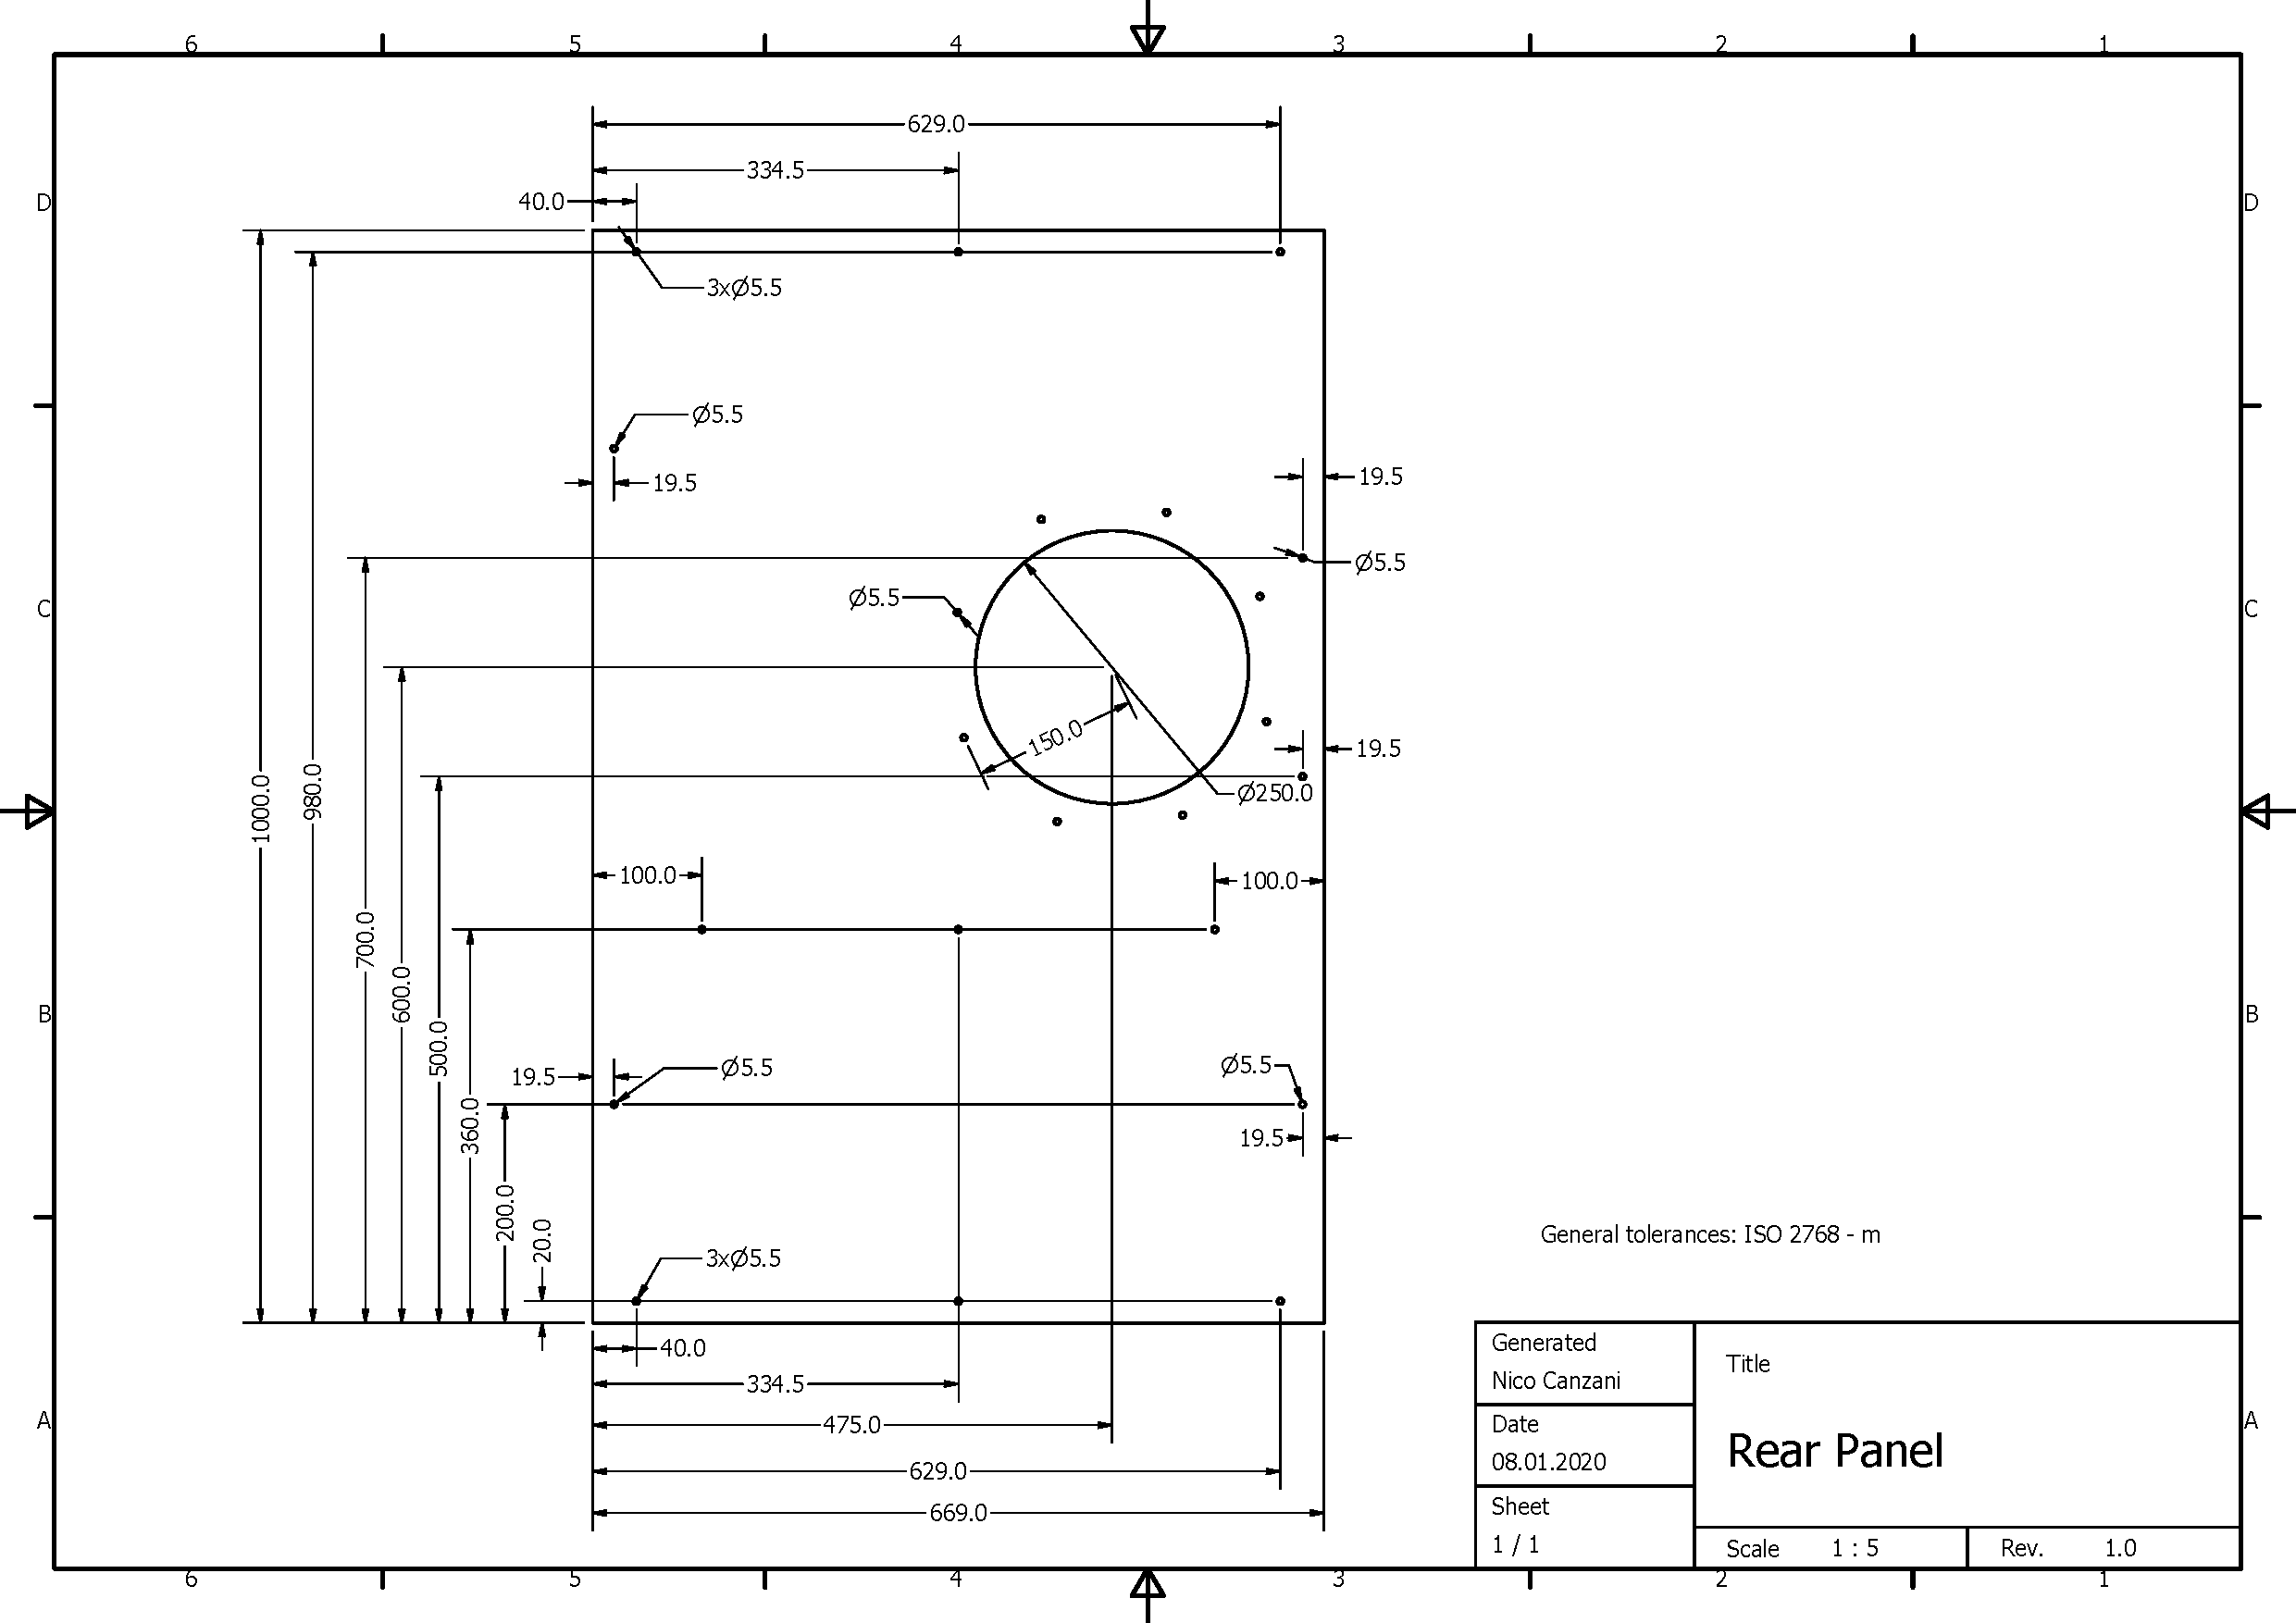
\includepdf[pages=-,landscape=true]{appendix/drawings_rear_panel.pdf}

  \section{Drawing Side Panel}
  \label{app:drawings_side_panel}
  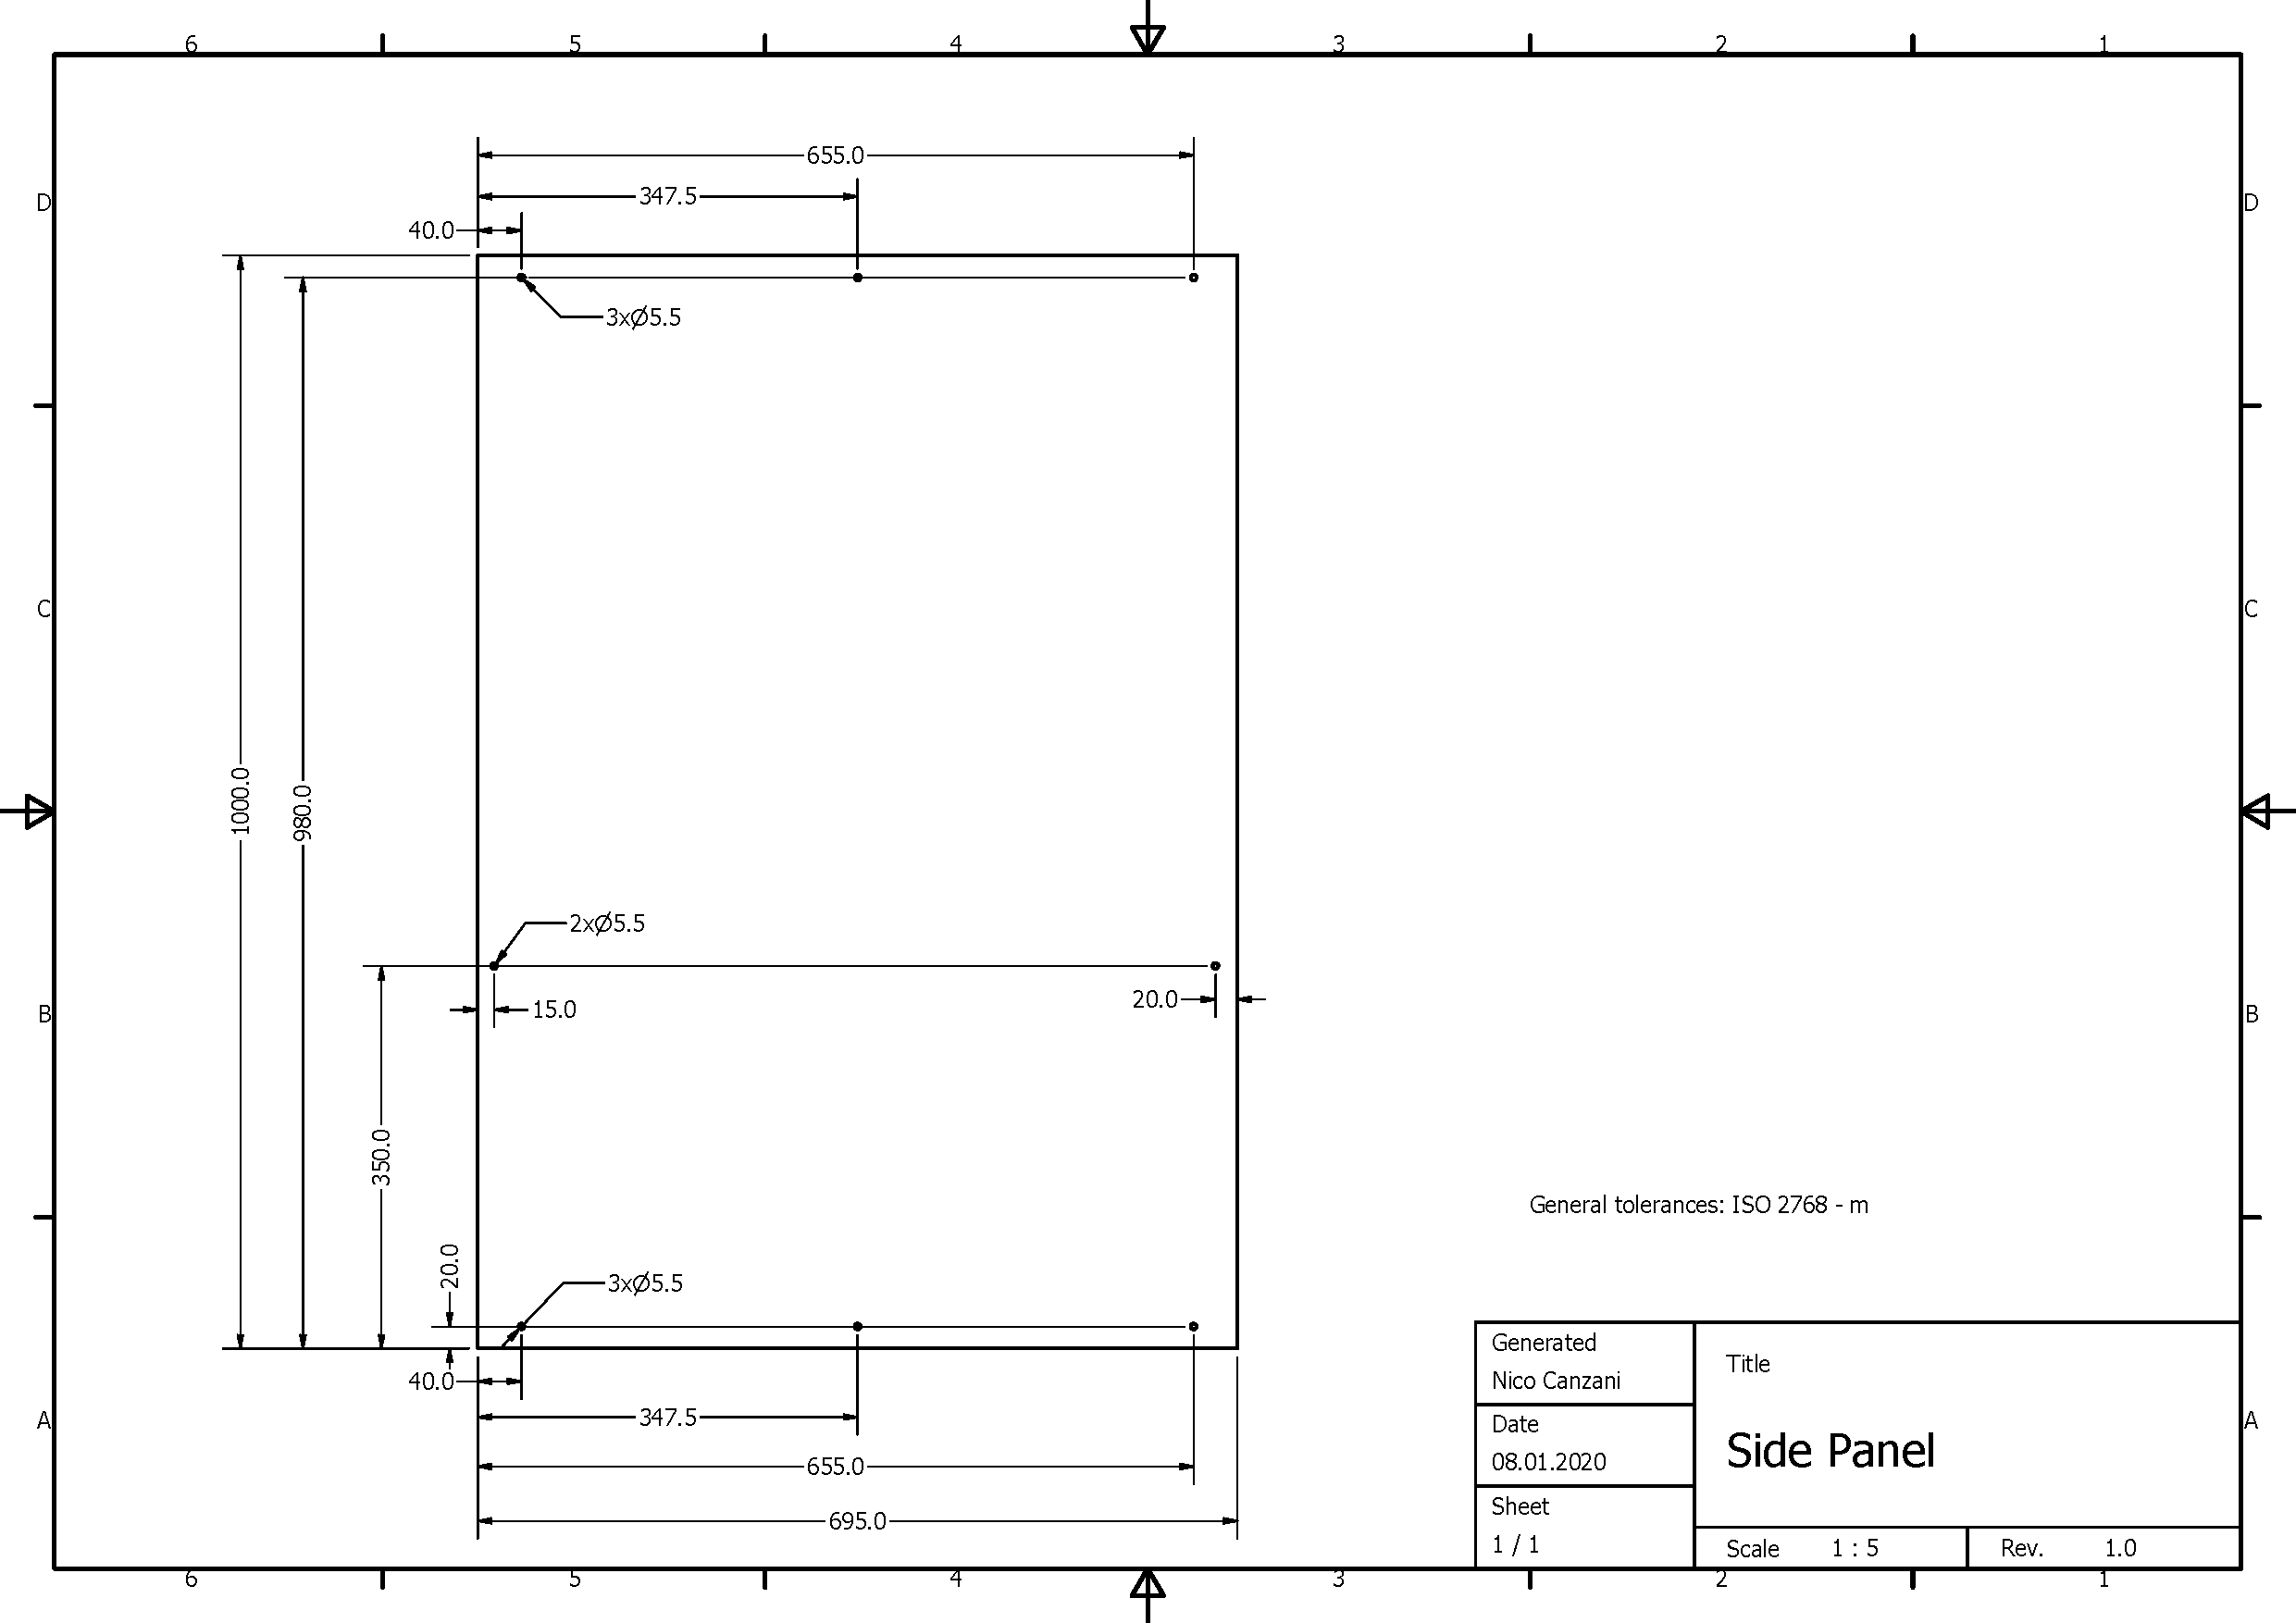
\includepdf[pages=-,landscape=true]{appendix/drawings_side_panel.pdf}

  \section{Throw Detection}
  \label{app:throw_detection}
  \lstinputlisting[style=C++]{appendix/throw_detection.cc}
\end{appendix}


% Debug
%\newpage
%\listoftodos[\section{To-Do}]
%\clearpage

\end{document}
